\section{Text Formatting}
Please use an 8.5-point Verdana font, or other sans serifs font as
close as possible in appearance to Verdana in which these guidelines
have been set. Arial 9-point font is a reasonable substitute for
Verdana as it has a similar x-height. Please use serif or
non-proportional fonts only for special purposes, such as
distinguishing \texttt{source code} text.

\subsubsection{Text styles}
The \LaTeX\ template facilitates text formatting for normal (for body
text); heading 1, heading 2, heading 3; bullet list; numbered list;
caption; annotation (for notes in the narrow left margin); and
references (for bibliographic entries). Additionally, here is an
example of footnoted\footnote{Use footnotes sparingly, if at all.}
text. As stated in the footnote, footnotes should rarely be used.

% \begin{figure}
%   
\includegraphics[width=0.9\columnwidth]{figures/sigchi-logo}
%   \caption{Insert a caption below each figure.}~\label{fig:sample}
% \end{figure}

\subsection{Language, style, and content}
The written and spoken language of SIGCHI is English. Spelling and
punctuation may use any dialect of English (e.g., British, Canadian,
US, etc.) provided this is done consistently. Hyphenation is
optional. To ensure suitability for an international audience, please
pay attention to the following:

\begin{table}
  \centering
  \begin{tabular}{l r r r}
    % \toprule
    & & \multicolumn{2}{c}{\small{\textbf{Test Conditions}}} \\
    \cmidrule(r){3-4}
    {\small\textit{Name}}
    & {\small \textit{First}}
      & {\small \textit{Second}}
    & {\small \textit{Final}} \\
    \midrule
    Marsden & 223.0 & 44 & 432,321 \\
    Nass & 22.2 & 16 & 234,333 \\
    Borriello & 22.9 & 11 & 93,123 \\
    Karat & 34.9 & 2200 & 103,322 \\
    % \bottomrule
  \end{tabular}
  \caption{Table captions should be placed below the table. We
    recommend table lines be 1 point, 25\% black. Minimize use of
    table grid lines.}~\label{tab:table1}
\end{table}

\begin{itemize}\compresslist%
\item Write in a straightforward style. Use simple sentence
  structure. Try to avoid long sentences and complex sentence
  structures. Use semicolons carefully.
\item Use common and basic vocabulary (e.g., use the word ``unusual''
  rather than the word ``arcane'').
\item Briefly define or explain all technical terms. The terminology
  common to your practice/discipline may be different in other design
  practices/disciplines.
\item Spell out all acronyms the first time they are used in your
  text. For example, ``World Wide Web (WWW)''.
\item Explain local references (e.g., not everyone knows all city
  names in a particular country).
\item Explain ``insider'' comments. Ensure that your whole audience
  understands any reference whose meaning you do not describe (e.g.,
  do not assume that everyone has used a Macintosh or a particular
  application).
\item Explain colloquial language and puns. Understanding phrases like
  ``red herring'' requires a cultural knowledge of English. Humor and
  irony are difficult to translate.
\item Use unambiguous forms for culturally localized concepts, such as
  times, dates, currencies, and numbers (e.g., ``1-5- 97'' or
  ``5/1/97'' may mean 5 January or 1 May, and ``seven o'clock'' may
  mean 7:00 am or 19:00). For currencies, indicate equivalences:
  ``Participants were paid {\fontfamily{txr}\selectfont \textwon}
  25,000, or roughly US \$22.''
\item Be careful with the use of gender-specific pronouns (he, she)
  and other gender-specific words (chairman, manpower,
  man-months). Use inclusive language (e.g., she or he, they, chair,
  staff, staff-hours, person-years) that is gender-neutral. If
  necessary, you may be able to use ``he'' and ``she'' in alternating
  sentences, so that the two genders occur equally
  often~\cite{Schwartz:1995:GBF}.
\item If possible, use the full (extended) alphabetic character set
  for names of persons, institutions, and places (e.g.,
  Gr{\o}nb{\ae}k, Lafreni\'ere, S\'anchez, Nguy{\~{\^{e}}}n,
  Universit{\"a}t, Wei{\ss}enbach, Z{\"u}llighoven, \r{A}rhus, etc.).
  These characters are already included in most versions and variants
  of Times, Helvetica, and Arial fonts.
\end{itemize}

% \begin{figure}
%   \includegraphics[width=.9\columnwidth]{figures/ea-figure2}
%   \caption{If your figure has a light background, you can set its
%     outline to light gray, like this, to make a box around
%     it.}\label{fig:bats}
% \end{figure}

% \begin{marginfigure}[-35pc]
%   \begin{minipage}{\marginparwidth}
%     \centering
%     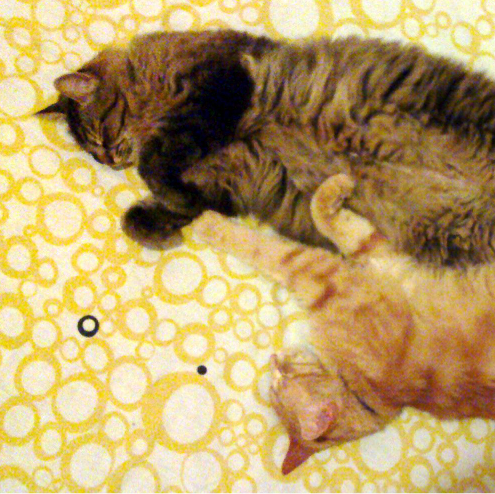
\includegraphics[width=0.9\marginparwidth]{figures/cats}
%     \caption{In this image, the cats are tessellated within a square
%       frame. Images should also have captions and be within the
%       boundaries of the sidebar on page~\pageref{sec:sidebar}. Photo:
%       \cczero~jofish on Flickr.}~\label{fig:marginfig}
%   \end{minipage}
% \end{marginfigure}
